\documentclass[11pt]{article}
\usepackage[pdftex]{graphicx}
\usepackage[explicit]{titlesec}
\usepackage[OT1]{fontenc}
\usepackage[most]{tcolorbox}
\usepackage[final]{pdfpages}
\usepackage[colorlinks=true, urlcolor=cyan, hyperfootnotes=false]{hyperref}
\usepackage{fullpage, graphicx, psfrag, url, caption, authblk, amsfonts, amsmath, amssymb, float, fancyhdr, multicol, cmbright, xcolor, amsthm, gensymb, physics}

\fancypagestyle{pages}{
	%Headers
	\fancyhead[L]{Physics 7A, Summer 2024 \\ Section 103}
	%\fancyhead[C]{\thepage}
	\fancyhead[R]{Discussion 5 \\ June 25}
\renewcommand{\headrulewidth}{0pt}
	%Footers
	%\fancyfoot[L]{}
	\fancyfoot[C]{}
	\fancyfoot[R]{\thepage}
\renewcommand{\footrulewidth}{0pt}
}

\newcommand\blfootnote[1]{
    \begingroup
    \renewcommand\thefootnote{}\footnote{#1}
    \addtocounter{footnote}{-1}
    \endgroup
}

\newcommand{\fig}[4]{
    \begin{figure}[H]
        \centering
        \includegraphics[scale={#3}, angle={#4}]{#1}
        \caption{#2}
        \label{exp4fit}
    \end{figure}
}

\newtheoremstyle{gangnamstyle}{}{}{}{}{\sffamily\bfseries}{.}{ }{}
\tcolorboxenvironment{definition}{boxrule=0pt,boxsep=0pt,colback={blue!10},left=8pt,right=8pt,enhanced jigsaw, borderline west={2pt}{0pt}{blue},sharp corners,before skip=10pt,after skip=10pt,breakable}
\tcolorboxenvironment{example}{boxrule=0pt,boxsep=0pt,colback={orange!10},left=8pt,right=8pt,enhanced jigsaw, borderline west={2pt}{0pt}{orange},sharp corners,before skip=10pt,after skip=10pt,breakable}
\tcolorboxenvironment{problem}{boxrule=0pt,boxsep=0pt,colback={cyan!10},left=8pt,right=8pt,enhanced jigsaw, borderline west={2pt}{0pt}{cyan},sharp corners,before skip=10pt,after skip=10pt,breakable}
\theoremstyle{gangnamstyle}{\newtheorem{definition}{Definition}[]}
\theoremstyle{gangnamstyle}{\newtheorem{example}{Example}[]}
\theoremstyle{gangnamstyle}{\newtheorem{problem}{Problem}[]}

\headheight=0pt
\footskip=0pt
\setlength{\oddsidemargin}{0 in}
\setlength{\evensidemargin}{0 in}
\setlength{\topmargin}{-0.5 in}
\setlength{\textwidth}{6.5 in}
\setlength{\textheight}{8.5 in}
\setlength{\headsep}{0.75 in}
\setlength{\parindent}{0 in}
\setlength{\parskip}{0.1 in}

\begin{document}
\normalfont
\pagestyle{pages}

% Begin Document

\begin{center}
\vspace{3in}
{\Large Discussion 5 } \\ [0.05in]
Dynamics \\ [-0.5in]
\end{center}

\section*{Topics}
Forces, Newton's Laws of Motion

\section{Review}

\begin{itemize}
\item Physical quantities: \\
A \textbf{Force} is an influence that causes an object to change its velocity. \\
The \textbf{Mass} of an object is the tendency to resist a change in its velocity. \\
Although these definitions seem recursive, they will be made clear through Newton's Second Law of Motion. 

\item Newton's Laws of Motion: \\
\textbf{1.} The velocity of an object remains constant if no net force acts on it. 
\[ \sum \Vec{F} = 0 \implies \Delta \Vec{v} = 0 \]
\textbf{2.} The net force on an object is proportional to its acceleration. The proportionality constant is the object's mass. 
\[ \sum \Vec{F} = m\Vec{a} \]

\item Common forces that you've seen so far: \\
\textbf{1.} Constant gravitational force $\Vec{F}_g$ (or weight $\Vec{W}$) on the surface of Earth: 
\[ \Vec{F}_g = m\Vec{g} \]


\textbf{2.} The normal force $\Vec{F_N}$ (or $\Vec{N}$) exerted by a surface in contact with an object. The normal force is responsible for supporting the object on top of the surface. 

\fig{figs/0625/normal.png}{Balance between Gravity and Normal Forces for a Stationary Box}{0.65}{0}

\textbf{3.} The tension force $\Vec{F}_T$ (or $\Vec{T}$) from a tout rope, which pulls on the objects connected on both sides. 
\fig{figs/0625/pull.png}{Rope and Blocks}{0.5}{0}
\fig{figs/0625/pullfbd.png}{Rope and Blocks, Free Body Diagram}{0.5}{0}


\item Common Mechanical Components: \\
\textbf{1.} A \textit{massless} string exerts a tension force of the same magnitude that pulls the objects on both sides, essentially transmitting the force from one end to the other. In the example above, if the cord was massless, $F_{AT}$ would be equal to $F_{BT}$. 

\textbf{2.} A \textit{massless and frictionless} pulley transmits the force through the rope in a different direction. In the example below, the rope wraps around the pulley and pulls both blocks $1$ and $2$ upward. 
\fig{figs/0625/pulley.png}{Blocks and Pulley}{0.6}{0}

\pagebreak

\item In solving problems in mechanics, it is essential to draw \textbf{free-body diagrams (FBDs)} for every object we analyze, showing all the forces acting on that object. We then use this diagram to apply Newton's Second Law in every Cartesian direction ($x$, $y$, and $z$) for that object. \\

For now, we can treat objects as point masses in FBDs. However, when you study rotational motion later in this class, you would need to draw \textbf{extended free-body diagrams}, where we specify the shape of the objects and draw the force vectors at where they are applied. 

\fig{figs/0625/fbd.png}{Examples of Free-Body Diagrams}{0.6}{0}

Here, regular FBDs are drawn for the masses, and an Extended FBD is drawn for the pulley.

\end{itemize}

\pagebreak

\section{Problems}

\textbf{1.} \textit{Morin, Introduction to Classical Mechanics, Problem 1.1} \\
A mass $m$, held up by two strings, hangs from a ceiling, as shown in Fig. 1.18. The strings form a right angle. In terms of the angle $\theta$ shown, what is the tension in each string?
\fig{figs/0625/morin11.png}{Morin, Problems 1.1}{0.75}{0}
\vspace{1.35 in}

\textbf{2.} \textit{Kleppner and Kolenkow, An Introduction to Mechanics, Problem 2.2} \\
The two blocks $M_1$ and $M_2$ shown in the sketch are connected by a string of negligible mass. If the system is released from rest, find how far block $M_1$ slides in time t. Neglect friction. 
\fig{figs/0625/kk22.png}{Kleppner and Kolenkow, Problems 2.2}{0.5}{0}

\pagebreak

\textbf{3.} \textit{Kleppner and Kolenkow, An Introduction to Mechanics, Problem 2.12} \\
A painter of mass $M$ stands on a scaffold of mass $m$ and pulls himself up by two ropes which hang over pulleys, as shown. He pulls each rope with force $F$ and accelerates upward with a uniform acceleration $a$. Find $a$—neglecting the fact that no one could do this for long.
\fig{figs/0625/kk212.png}{Kleppner and Kolenkow, Problems 2.12}{0.6}{0}

\pagebreak

\textbf{4.} \textit{Giancoli, Physics for Scientists and Engineers, Problem 4.76} \\
A block (mass $m_A$) lying on a fixed frictionless inclined plane is connected to a mass $m_B$ by a cord passing over a pulley. The cord and the pulley are massless. \\
(a) Determine a formula for the acceleration of the system in terms of $m_A$, $m_B$, $\theta$, and $g$. \\
(b) What conditions apply to masses $m_A$ and $m_B$ for the acceleration to be in one direction (say, $m_A$ down the plane), or in the opposite direction? 
\fig{figs/0625/giancoli476.png}{Giancoli, Problems 4.76}{0.6}{0}

\pagebreak

\textbf{5.} \textit{Giancoli, Physics for Scientists and Engineers, Problem 4.78} \\
The masses $m_A$ and $m_B$ slide on the smooth (frictionless) fixed inclines as shown. \\
(a) Determine a formula for the acceleration of the system in terms of $m_A$, $m_B$, $\theta_A$, $\theta_B$, and $g$. \\
(b) What ratio, $m_A / m_B$, would allow the masses to move at constant speed along their ramps in either direction?
\fig{figs/0625/giancoli478.png}{Giancoli, Problems 4.78}{0.75}{0}

\pagebreak

\textbf{6.} \textit{Kleppner and Kolenkow, An Introduction to Mechanics, Problem 2.7} \\
A pole of negligible mass leans against a wall, at angle $\theta$ with the horizontal. Gravity is directed down. \\
a) Find the relationship between the vertical acceleration of the top left end and the horizontal acceleration of the bottom right end. \\
\textit{Hint: Relate the width and height of the triangle using Pythagorean Theorem. Differentiate twice with respect to time.} \\
b) Now suppose that each end carries a pivoted mass $M$. Find the initial vertical and horizontal components of acceleration as the pole just begins to slide on the frictionless wall and floor. Assume that at the beginning of the motion, the forces exerted by the rod are along the line of the rod.
\fig{figs/0625/kk27.png}{Kleppner and Kolenkow, Problems 2.7}{0.6}{0}

\vspace{3.25 in}
\textbf{7.} Problem from past Physics 7A Exam (Next Page) \\
\textit{Hint: The total length of the string is constant: (For part d) Use this condition to write an equation involving positions that equals to a constant, then differentiate that equation.}

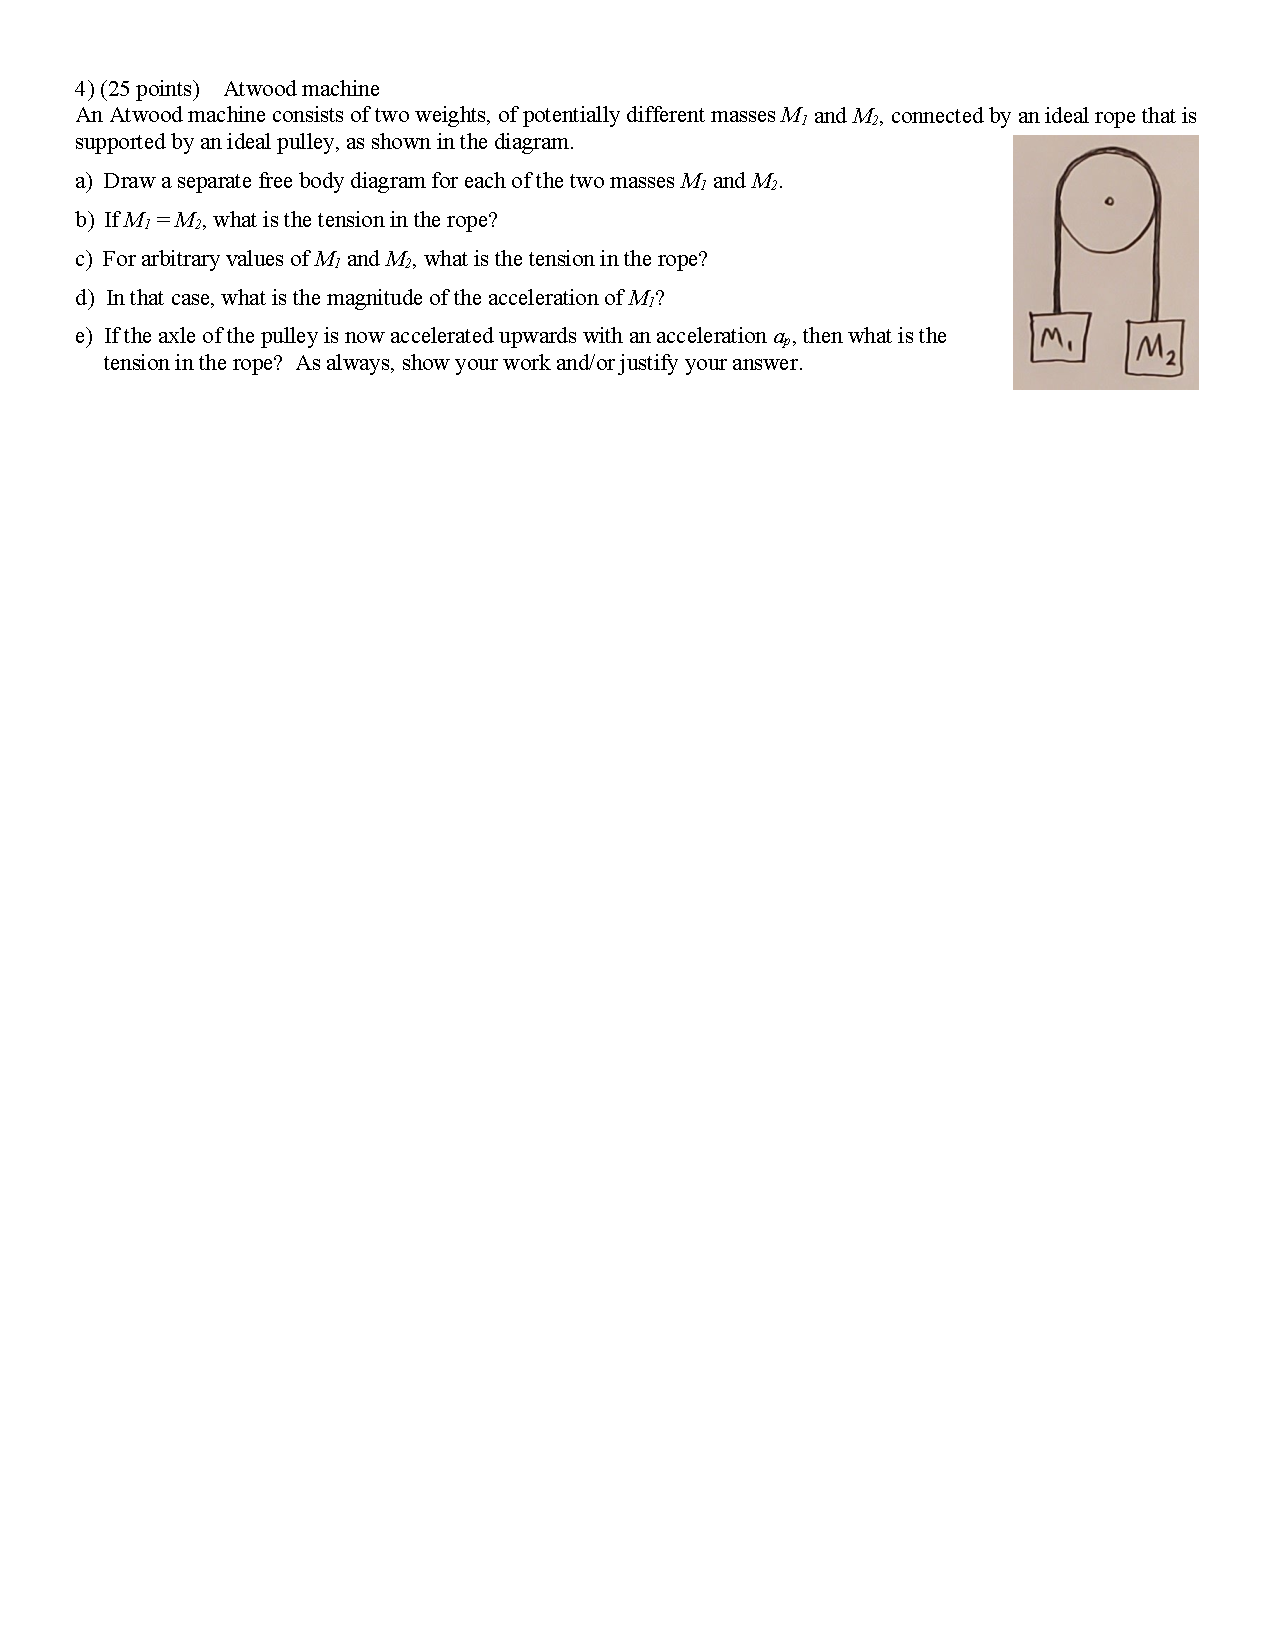
\includepdf[pages=-]{figs/0625/atwood.pdf}

\textbf{8.} \textit{Kleppner and Kolenkow, An Introduction to Mechanics, Problem 2.8} \\
Masses $M_1$ and $M_2$ are connected to a system of strings and pulleys as shown. The strings are massless and inextensible, and the pulleys are massless and frictionless. Find the acceleration of $M_1$. \\
\textit{Hint: Define a variable $y_3$ for the position of the bottom pulley. The total length of each string is constant: Use this condition to write an equation involving positions that equals to a constant, then differentiate that equation.}
\fig{figs/0625/kk28.png}{Kleppner and Kolenkow, Problems 2.8}{0.6}{0}

\pagebreak

\textbf{9.} \textit{Morin, Introduction to Classical Mechanics, Problem 2.4, 2.5} \\
a) A massless pulley hangs from a fixed support. A massless string connecting
two masses, $m_1$ and $m_2$, hangs over the pulley (see Fig. 2.23). Find the acceleration of the masses and the tension in the string. \\
b) A double Atwood’s machine is shown in Fig. 2.24, with masses $m_1$, $m_2$, and $m_3$. Set up a system of equations that can be used to solve for the accelerations of the masses. If time permits, solve it. 
\fig{figs/0625/morin245.png}{Morin, Problems 2.4, 2.5}{0.75}{0}

\end{document}
